\section{Introduction}
The movie industry continues to grow year on year, with increasing competition between movie producers and film companies to boost revenue and increase ratings. The performance of a movie at the box office is influenced by a host of factors, some of which include the cast, budget, time of release and director involved. This makes predicting the box office of movies very challenging. Quite a number of studies, however, have been done by researchers attempting to identify the influential factors and predict the box office of movies \cite{sharda2006predicting}. Most of the studies failed to build models with high predicting accuracy that can serve as guidelines for decision making process. Most of the literature on this problem can be classified into two categories i) predicting the gross prior to movie release; ii) predicting the gross after the movie release. Models built in the second category generally have higher precision as more predictive variables including first week box office and word-of-mouth effects are provided. Besides, all the studies turned this problem into classification problem as the value of movie gross is very sparse.  And many traditional statistical methods and artificial neural network (ANN) were applied. Among those methods, ANN performed the best with highest accuracy under the same experimental conditions \cite{sharda2006predicting}.
 
The aim of our study is to apply different kinds of predictive data mining techniques including classification and regression and try to find the best model. What differentiates our study from the others is that we first built a classification model and then used the predicting results of the classification model as new features for regression models. Results show there is a 6.6\% increase in regression model accuracy.

\section{Materials and methods}

\subsection{IMDB dataset}
The dataset used was the IMDB 5000 Movie Dataset hosted on Kaggle \footnote{https://www.kaggle.com/deepmatrix/imdb-5000-movie-dataset}. It has the data for 5044 movies, ordered by the highest grossing values and it provides 28 features. Features range from binary values (colour or black and white), textual (director and actor names, genre, country of origin) as well as numerical values (gross, number of likes on social media, release year).  However, the dataset has several limitations, one of which is missing values. For this reason, we performed the scraping process again to improve the dataset and collect more data that was originally available.

\subsubsection{Re-scraping}
First, up-to-date budget values were sourced from the-numbers.com, which provides a database of production and marketing budgets for movies, as well as domestic and worldwide gross values. The original dataset only included the domestic gross estimates from IMDB.com. As the worldwide gross is the target value  being predicted, extra focus was put on getting accurate data for this feature.

Secondly, based on the list of movies obtained in the first step, the script obtained the IMDB links for the movies, using fuzzy matching  to resolve naming ambiguities (some movies have several names that identify them, eg. Fast \& Furious 6 and Furious 6), and scraped IMDB for the available data. Additionally, the script queried Facebook for popularity measures, count of likes for actors, movies and directors.

\subsubsection{Dataset joining}
Finally, data from all steps, the-numbers.com, IMDB and Facebook, was joined in a single dataset ordered by highest grossing movies. The main contribution of this step was the correction of worldwide gross values. Additionally, all values were converted to a common currency (USD), as the original dataset reported gross values in local currencies. This was particularly important for currencies that have low exchange rate to USD, like South Korean Won, as they inflate the values.

\subsection{Feature engineering}
Since our goal is to predict box-office revenue before the movie premiere, the first step was to remove the features that are not available before the release of the movie. Those include \textit{imdb\_score, movie\_facebook\_likes, num\_critic\_for\_reviews, \\num\_user\_for\_reviews, num\_voted\_users}.

After obtaining the updated dataset, additional work was performed manually to clean and enhance the data. Duplicates were removed, and additional columns were added, like ‘blockbuster’, which designated if the movie released during Christmas or Summer season (June/July/August/December), as well as manual fixing of duration, countries, and similar values that show outliers. These tasks were performed in OpenRefine\footnote{http://openrefine.org}.

\subsubsection{Data transformations}
\label{sec:data_trans}
Additionally, in cases where there is a lot of differences in variation in a dataset, data can be classified as heteroscedastic. Logarithmic transformation is usually applied in those situations \cite{kvalheim1994preprocessing}. Given that the ranges for the worldwide gross are several orders of magnitude, from hundreds of thousands of dollars, all the way to billions, logarithmic transform in this case solves the issue. In the pipeline process, several other transformations were applied as well, like standardisation, normalisation and polynomial transformation. 

Finally, we applied vectorization of categorical data. Results were compared to find the combination of transformers that provides the best scores. The resulting combination was the following: count vectoriser was used for name values (actors and directors) and term-frequency was applied to categorical values (like colour, countries, genres). The differences between different approaches are minor, less than 1\% (second best combination was 0.73\% less accurate, it used count vectoriser for names and term-frequency/inverse-document-frequency for categorical values), but still affect the end model so it was important to find the best performing transformations.


\subsection{EXPLORATORY DATA ANALYSIS (EDA)}
We applied EDA to understand the nature of the data, bivariate relationships and discover patterns that can guide the selection and application of prediction machine learning techniques \cite{behrens1997principles}. \figurename{} \ref{fig:hist}(a) shows that gross variable is not normally distributed. As mentioned in Section \ref{sec:data_trans} it is useful to use the logarithmic transformation to deal with a more normally distributed version of this variable. See \figurename{} \ref{fig:hist}(b). A similar exploration analysis was applied on the other variables using the common visualization tools, including pairwise plots and correlations matrix. Correlation analysis revealed that gross and budget are positively correlated (correlation coefficient of 0.74), and that there is not a significant correlation between the movie gross and the other explanatory variables. \figurename{} \ref{fig:scatter}, which presents a scatter plot of the two most relevant variables in their original and log transformed form, illustrate that these variables are highly heteroscedastic, and therefore apropiate transformations should be considered in the pipeline.
\begin{figure}[h]
\centering
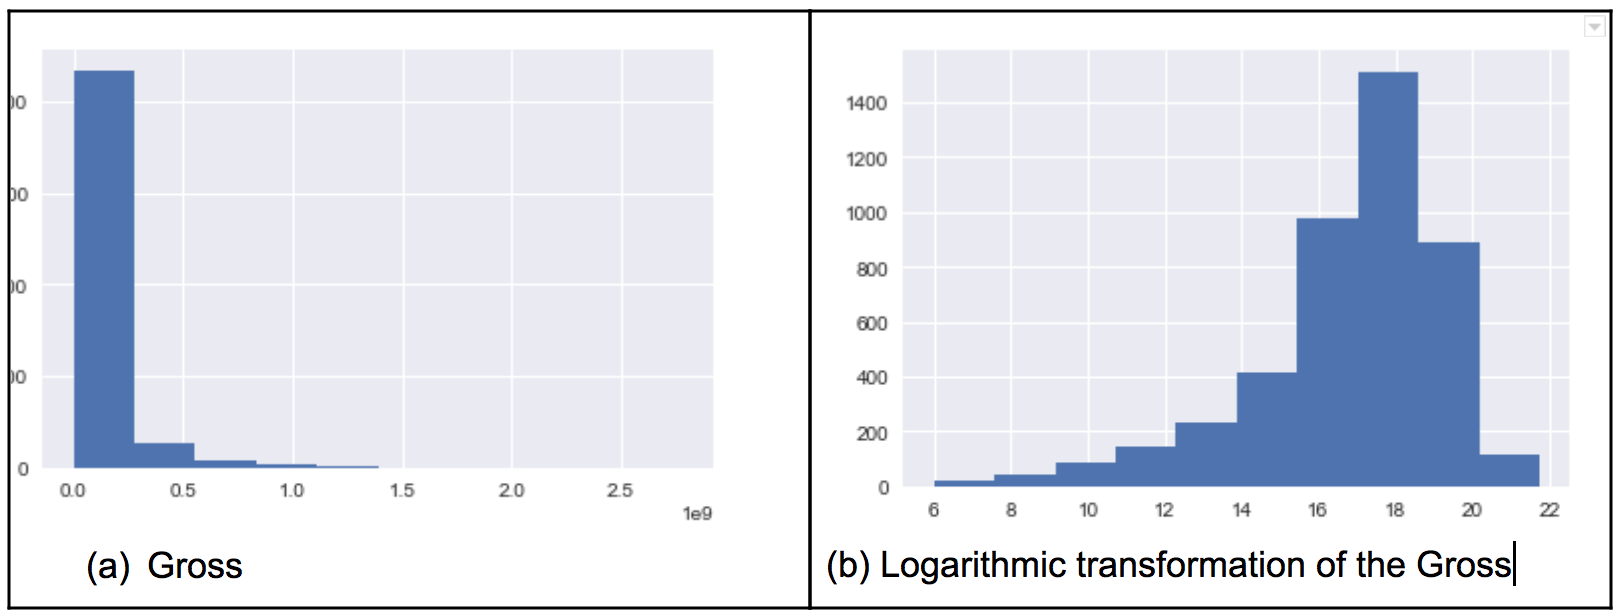
\includegraphics[width=3.2in]{figures/hist}
\caption{Histograms of the gross variable} 
\label{fig:hist}
\end{figure}
\begin{figure}[h]
\centering
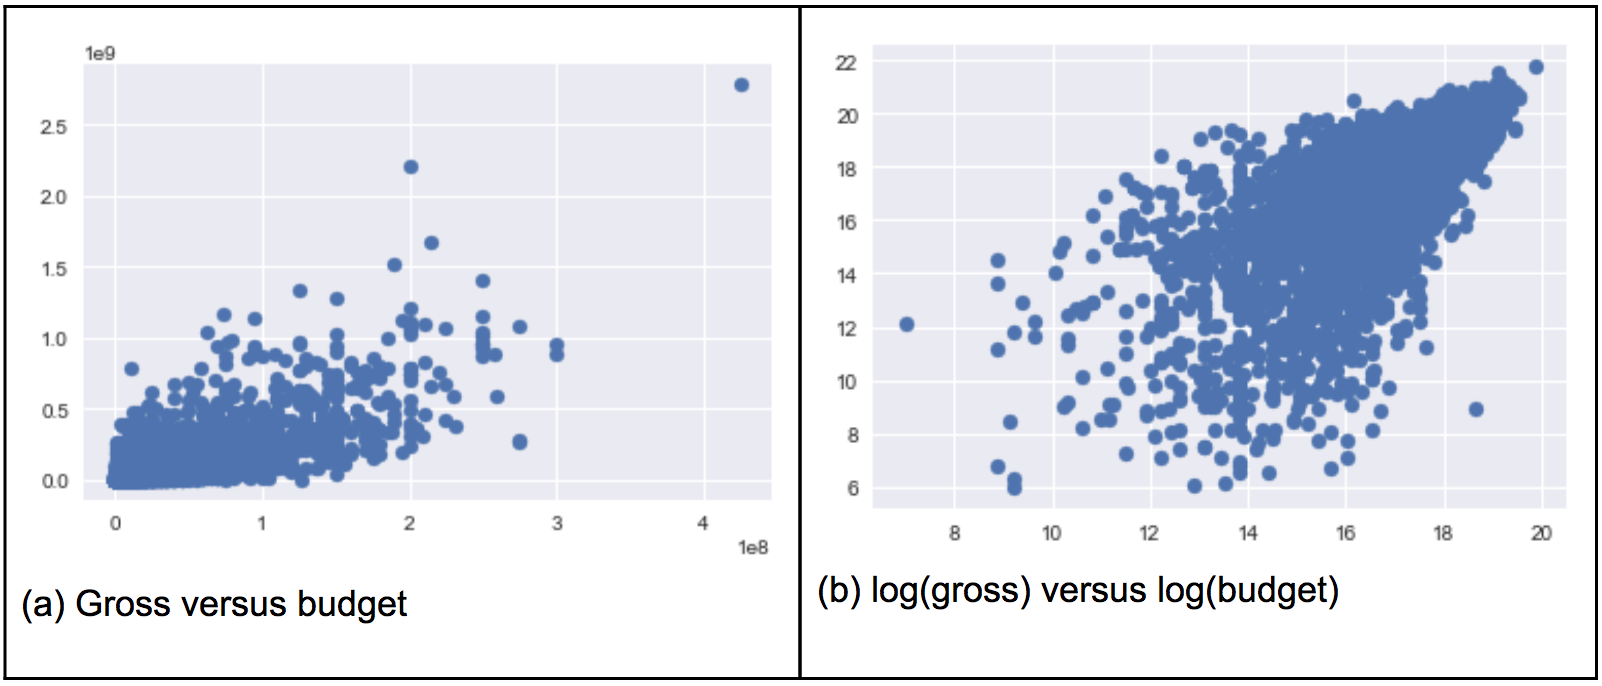
\includegraphics[width=3.2in]{figures/scatter}
\caption{Scatter plot of the gross versus the budget} 
\label{fig:scatter}
\end{figure}

\subsubsection{DIMENSIONALITY REDUCTION}
A plot of the cumulative explained variance plot created by means of PCA over the processed dataset is shown in \figurename{} \ref{fig:variance}, emphasising that there is not a small subset of variables that can explain the majority of variance in the data. In other words, we need about 125 variables (out of 184) to explain 80\% of the variation. This suggests that there is not much space for dimensionality reduction in this dataset.

\begin{figure}[h]
\centering
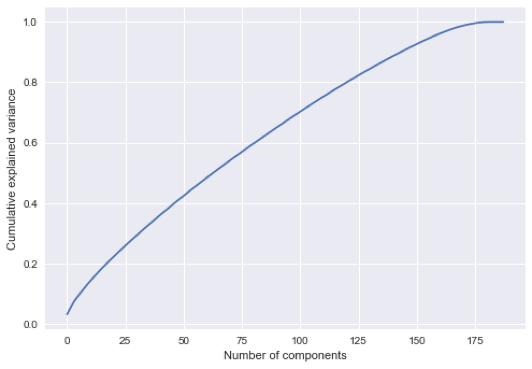
\includegraphics[width=3.2in]{figures/variance}
\caption{Explained variance plot} 
\label{fig:variance}
\end{figure}

Dimensionality reduction is also useful to create a visual representation of multidimensional data in a reduced space. For instance, \figurename{} \ref{fig:pca} shows a PCA-reduced 3D representation of the dataset studied in this report. It can be seen that most of the observations are scarcely scattered in a certain area of the plot, but also there is a considerable amount of points scattered outside that area. The plot also shows that there is not clear evidence of clusters. 

\begin{figure}[h]
\centering
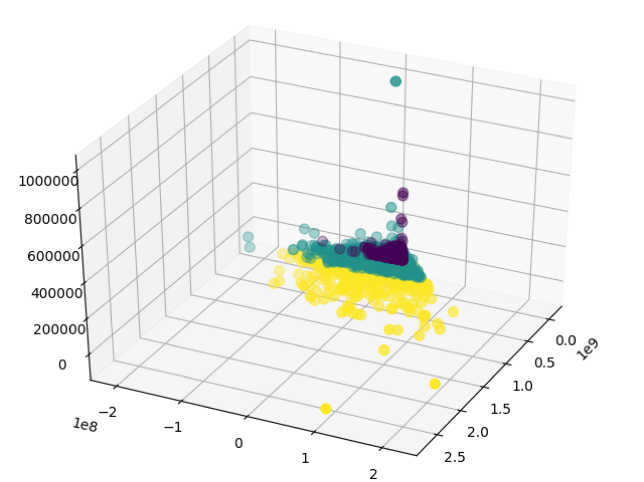
\includegraphics[width=3.2in]{figures/pca}
\caption{PCA-reduced 3D visualization of the dataset. The color of the points represent a three-level category of the gross.} 
\label{fig:pca}
\end{figure}

Regarding feature selection, we tried several methods such as variance threshold, recursive feature elimination, and feature selection based on models. As expected, all these methods agree that the most important variables are the numeric variables. However, they differ in which of the binary variables are the most relevant.

\subsection{Approach}
We aimed to find the most accurate model among dozen different machine learning techniques including linear models, ensemble methods, support vector machines (SVM) and neural nets.  Each model requires a careful parameter optimization to find the best fitting model. 
 
To solve the model selection and optimization, we developed a framework built on top of sklearn that allows to define a workflow composed of features transformation, model training, validating and testing. To integrate and automate this workflow, we used  pipeline and GridSearchCV functions of sklearn \cite{sklearnpipeline}. The pipeline allows us to set parameters for the models in each step while chaining them together without keeping track of the data. GridSearchCV allows us to construct a grid of the parameter combinations and search for the best one. Besides, it also automatically performs cross-validation on each model for each combination. In the end, it returns the best model with the according parameters. However this functionality was not sufficient to automate the testing of different machine learning models, therefore extra functionality was implemented to support it.

To solve the model selection and optimization, a  workflow has been applied which consists of features transformation, model training, validating and testing. To integrate and automate this workflow, we used  pipeline and GridSearchCV functions and sklearn \cite{sklearnpipeline}. The pipeline allows us to set parameters for the models in each step while chaining them together without keeping track of the data. GridSearchCV allows us to construct a grid of the parameter combinations and search for the best one. Besides, it also automatically performs cross-validation on each model for each combination. In the end, it returns the best model with the accompanying parameters. However this functionality was not sufficient to automate the testing of different machine learning models, therefore extra functionality was implemented to support it.

The price of these benefits, however, is in the form of computation time. A pipeline trying different pre-processing, transformation, reducers, and parameter grids,  can take from several hours up to days to complete. 
\subsection{Regression}

A number of regression techniques were applied to the problem via the pipeline, with varying results. Based on insights from our experimentation, focus was placed on one regression technique: Gradient Boosting Regression. This section describes in detail the application of this ensemble method in predicting gross values of movies. 

\subsubsection{Gradient Boosting Regression}
Gradient Boosting was applied on the data, with least squares as the error function. The best result was produced with a Gradient Boosting Regressor with 1000 base learners and a corresponding low learning rate of 0.1. Base learners in this case are decision trees which are used as weak learners in the gradient boosting process \cite{natekin2013gradient}. These are constructed in a greedy fashion, choosing the best split to minimize the loss. 

Given the high number of regression trees combined to form the Gradient Boosting model, a visual inspection of individual trees is hard to interpret. We look into feature importance to highlight features that would ordinarily be used frequently in split points in our model. It is found that the most important features for this model are the production budget, movie duration, and the total number of Facebook likes for the cast. The production budget, however, immensely outweighs the other features in terms of importance. 

To extend this further, we take a look at partial dependence plots to show the dependence between the target response and the most important set of features (i.e. the expected response as a function of the features). \figurename{} \ref{fig:gradient_boost_dependency} shows dependency plots for production budget and a two-way partial dependency plot of the former and the movie duration. The effect of the production budget on the gross can be seen in the first plot, with a clear linear relationship between them. The two-way plot shows the interactions between the production budget and movie duration, which are the two most important features as per the model. For a movie of a certain duration d, irrespective of whether high or low, its gross is strongly dependent on production budget.
\iffalse
\begin{figure}[h]
\centering
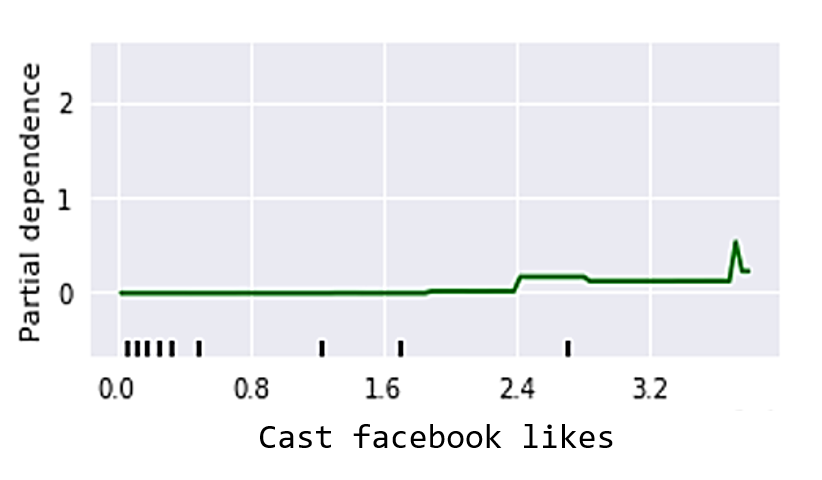
\includegraphics[width=3.2in]{figures/gb_dependency_1}
\label{fig:gradient_boost_dependency}
\end{figure}
\begin{figure}[h]
\centering
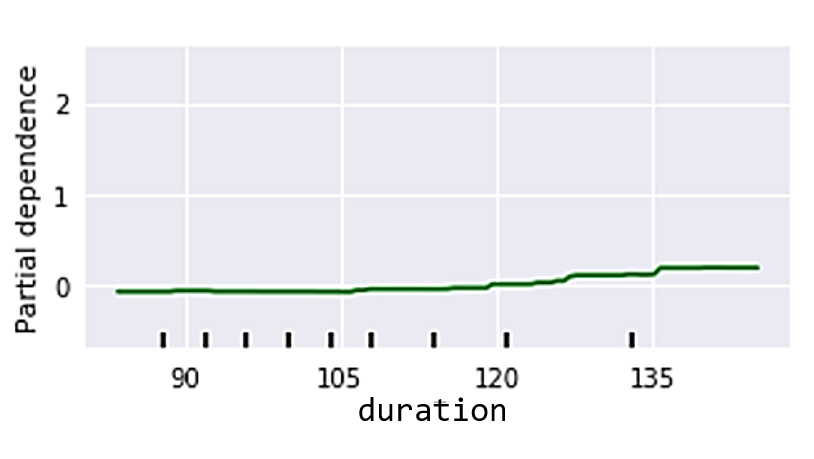
\includegraphics[width=3.2in]{figures/gb_dependency_2} 
\label{fig:gradient_boost_dependency}
\end{figure}
\fi
\begin{figure}[h]
\centering
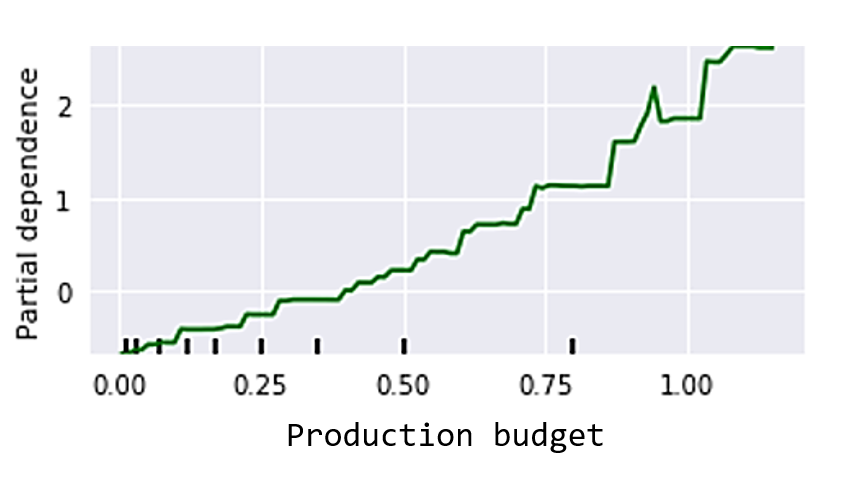
\includegraphics[width=3.2in]{figures/gb_dependency_3}
\label{fig:gradient_boost_dependency}
\end{figure}
\begin{figure}[h]
\centering
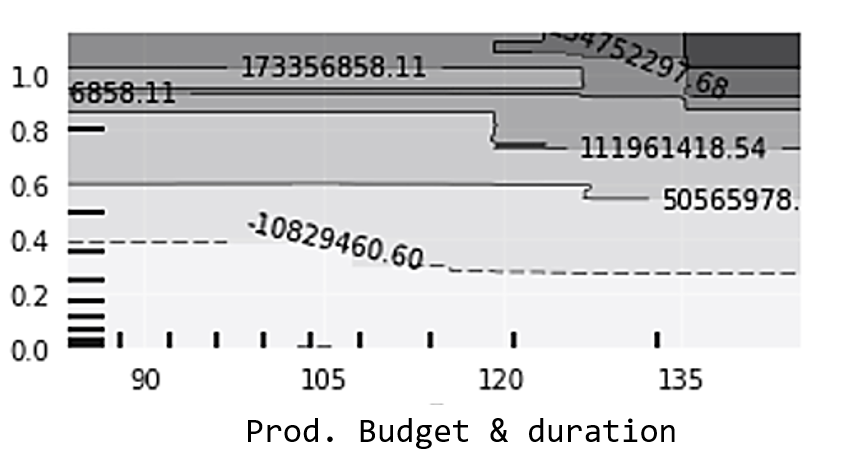
\includegraphics[width=3.2in]{figures/gb_dependency_4}
\caption{Dependency plots for Gradient Boosting Model} 
\label{fig:gradient_boost_dependency}
\end{figure}

We also plot a learning curve to provide some insight into training and validation scores for varying number of training samples. From \figurename{} \ref{fig:gradient_boost} it can be seen that the training and validation performance converge as the number of training samples increases. This indicates that addition of  more data is unlikely to help increase the validation performance as well as model generalisation to new data.

\begin{figure}[h]
\centering
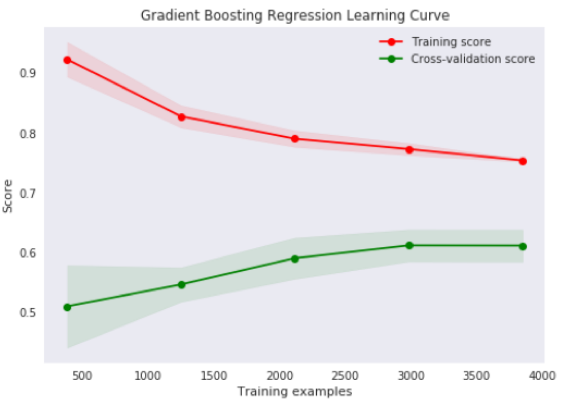
\includegraphics[width=3.0in]{figures/gradient_boost}
\caption{Gradient Boosting Regression Learning Curve} 
\label{fig:gradient_boost}
\end{figure}

\subsection{Classification}

Over a dozen different classifiers have been used within the pipeline. As result of experimentation, the pipeline was narrowed down to one classifier. This section discusses the optimization of parameters for selecting the right model to grow the decisions trees and constructing the ensembles to generalise a well fitted model, taking into account bias/variance trade-off \cite{biasvariance}. Overall, 9 different classification cases were attempted, ranging from classifying into 2 classes up to 10 classes of gross values. 

\subsubsection{Gradient Boosting Model Selection}
This section explores a model selection for 3 classes classifier.

\begin{figure}[h]
\centering
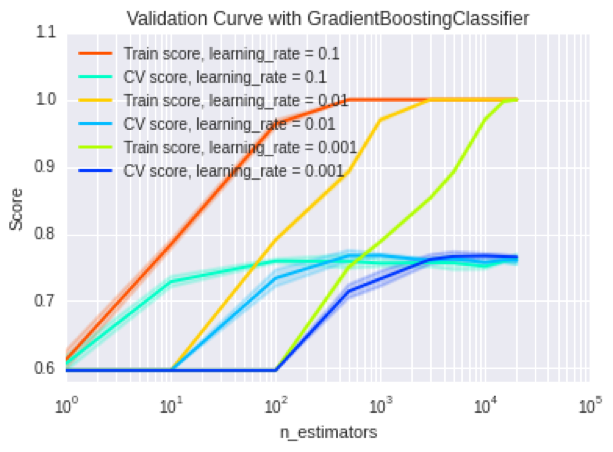
\includegraphics[width=3.0in]{figures/v_curve1}
\caption{GradientBoostingClassifier learning rate validation curves} 
\label{fig:gradient1}
\end{figure}

\begin{figure}[h]
\centering
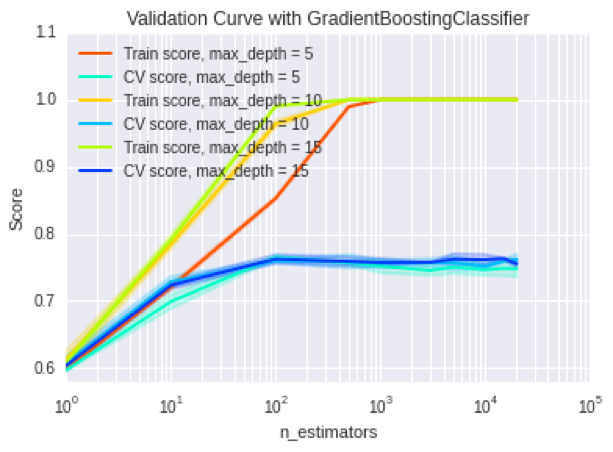
\includegraphics[width=3.0in]{figures/v_curve2}
\caption{GradientBoostingClassifier max depth validation curves}
\label{fig:gradient2}
\end{figure}

The learning rate/shrinkage represents the weight that is applied to the error minimization amount by each newly added decision tree \cite{biasvariance}. As a result, a smaller learning rate requires more estimators to be added in order to provide a more generalised model, as it can be seen in \figurename{} \ref{fig:gradient1}. Learning rate of 0.01 achieves the highest performance with a small amount of 500 ensembles and does not overcomplicate the model as 0.001 rate does. Max tree depth controls the maximum number of nodes within single tree, hence limiting number of decisions a single tree can take. A max depth of 10 achieves an optimal performance with 100 ensembles. It can be seen that a bigger increase does not increase validation accuracy and only complicates the learning. 

Other optimised features included ‘min\_samples\_per\_leaf’, that regulate the amount of samples necessary to fall within a node so that it becomes a leaf. Experimentation shows that having less than 3 samples per a leaf decreases the validation accuracy and leads to gain in variance.  Maximum features dictate the number of features to consider when classification tree looks for the best split in the samples provided in order to minimise the classification error \cite{tan2006classification}. The score of 0.1 of all features to be considered when split is produced was found to produce a better generalising model. Max\_leaf\_nodes determines how many leafs tree can have when it is constructed, hence controlling the amount of eventual decisions that are taken in the tree. No limit for the configuration indicates unlimited amount of leafs and it did display the optimal performance.  The analytical results coincide with findings of the parameters search over the pipeline, which is (max\_leaf\_nodes = None, learning\_rate = 0.1, max\_depth =  10, min\_samples\_leaf = 5, max\_features = 0.01,n\_estimators = 500).­ This model has a balance bias/variance ratio, which produces a good generalising model. It requires less estimators than the regression model as well, as its learning curve is faster and requires less complex model to generalise. Both models select the budget as most important feature, as seen in \figurename{} \ref{fig:gradient_boost_dependency}, followed by rest of the numerical features.


\subsection{Final Model}
\begin{figure}[h]
\label{fig:final_model}
\centering
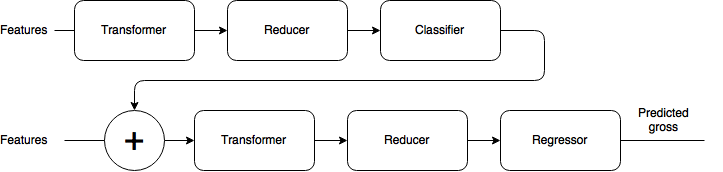
\includegraphics[width=3.2in]{figures/finalmodel1}
\caption{Final model 1}
\label{fig:model1}
\end{figure}
\begin{figure}[h]
\centering
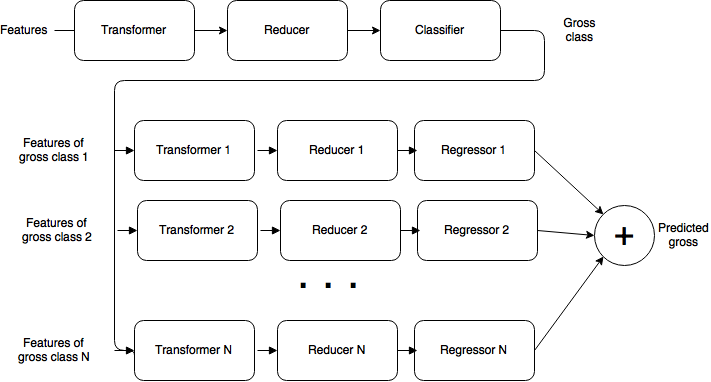
\includegraphics[width=3.2in]{figures/finalmodel2}
\caption{Final model 2}
\label{fig:model2}
\end{figure}
Two architectures were tested for the final model, which perform unification of classification and regression models, in order to improve regression accuracy. To optimize the model, a custom GridsearchCV function was written in order to support two models in a pipeline, unlike sklearn’s default of one. The first model trains a pipeline for the classification stage, which then concatenates its results with features for each data sample. Then a separate regression pipeline is trained from the concatenated samples, which then output final result.

The second model firstly is trained to classify all the samples and then for each set of classes produces an independent regression model. As a result, each gross class of samples uses a different optimized regression pipeline to find the final results.

The second model was found to perform worse, due to much smaller training data available and as it was seen before, a gradient boost regression requires over 3000 samples to achieve validation saturation, but the average set size of classified samples available for training each regression step  ranges from 1920 down to 427.

\section{Results}
The followings results have been obtained from feeding the data through the first architecture of the final model. The \tablename{} \ref{tab:top_ten_methods} contains results for 9 different classification cases. It has to be noted that the sole regression results are indicated for comparison purposes and the sole regression without class data fed in was not involved in generating the final result, whereas the classification results indicate the performance of the classification step of model, results of which are fed into the regression step.

\begin{table*}[!h]
\caption{Class - score of the classification stage. Reg - reference score of the best standalone regression model. Combo - the regression results of the combined final model. Train - training accuracy, Valid - Cross validation accuracy, Test - Testing Accuracy. The classification results are measures as a fraction of classes predicted right. Regression results are measured as a $R^2$ metric.}
\label{tab:top_ten_methods}
\centering
\begin{tabular}{|p{1cm}|p{1cm}|c|c|c|c|c|c|c|c|}
\hline
Classes&Class Train&Class Valid&Class Test&Reg Train&Reg Valid&Reg Test&Combo Train&Combo Valid&Combo Test \\
\hline
2 & 0.982 & 0.924 & 0.916 & 0.809 & 0.583 & 0.625 & 0.957 & 0.664 & 0.676 \\
3 & 0.872 & 0.761 & 0.771 & 0.809 & 0.583 & 0.625 & 0.906 & 0.669 & 0.691 \\ 
4 & 0.850 & 0.624 & 0.627 & 0.809 & 0.583 & 0.625 & 0.913 & 0.687 & 0.680 \\
5 & 0.868 & 0.536 & 0.549 & 0.809 & 0.583 & 0.625 & 0.723 & 0.690 & 0.670 \\
6 & 0.834 & 0.490 & 0.493 & 0.809 & 0.583 & 0.625 & 0.758 & 0.720 & 0.691 \\
7 & 0.839 & 0.461 & 0.479 & 0.809 & 0.583 & 0.625 & 0.772 & 0.746 & 0.679 \\
8 & 0.612 & 0.362 & 0.385 & 0.809 & 0.583 & 0.625 & 0.914 & 0.690 & 0.685 \\
9 & 0.642 & 0.356 & 0.377 & 0.809 & 0.583 & 0.625 & 0.844 & 0.700 & 0.681 \\
10 & 0.619 & 0.334 & 0.382 & 0.809 & 0.583 & 0.625 & 0.716 & 0.682 & 0.682 \\
\hline

\end{tabular}
\end{table*}

Class - score of the classification stage. Reg - reference score of the best standalone regression model. Combo - the regression results of the combined final model. Train - training accuracy, Valid - Cross validation accuracy, Test - Testing Accuracy. The classification results are measures as a fraction of classes predicted right. Regression results are measured as a $R^2$ metric. 

\section{Discussion}
Our test results show that we can forecast a final gross of a movie with 69.1\% accuracy when the final combinatory model is used. There are multiple class cases that equal this or get close to it, but only the case with 6 classification categories achieves a good general model. This case achieves 75.8\% training accuracy and 72\% cross validation score. Since these three scores are close in value, it indicates that model is neither under fitted or overfitted, and sits on an optimal point of the bias/variance tradeoff curve. Our combined model increases the sole regression validation and test performance by 13.8\%  and 6.6\% respectively. 

The gradient boosting has been found to be the best performing method for both classification and regression under same experimentation conditions (compared to Linear and Logistic regression, Support Vector Machines, Neural Networks). 

The the final combined model performs within 1-3\% test accuracy difference regardless of the amount of classes used for classification stage. Moreover the classification performance drops dramatically from 91.6\% to 38.2\% for 2 to 10 classes respectively, hence the final combined result could be expected to suffer. This is not the case due to fact that classes are arbitrary boundaries that were predefined, and the classifier model still classifies samples within the ranges it sees it fits the best. As result, all newly added classes simply fall within range of previous larger class cases, and most of the data gets classified into 3 different classes only. This has been observed to be the case via the analysing the performance plots.

In the data transformation parts of the pipeline we have experimented with multiple logarithmic and polynomial, as well as standardisation and  normalization transforms. We have found that the most meaningful transform  is the logarithmical budget transform, which decreases the heteroscedasticity and improves the result, due to the budget explaining the most variance in the gross. Standardisation has been proven to improve results by near negligible  amount, as when data samples are split by the decision trees, feature scaling does not affect split area selection \cite{chen2014introduction}. Moreover, it was found that prior features selection in the model improves result only by  2-3\%, due to the fact gradient boosted trees perform the features selection implicitly during the ensemble process, thereby it is redundant.

As shown earlier, the gradient boosted trees can be easily trained to have near 100\% train accuracy by adding more tree ensembles. Using small amount of data with big amount of ensembles leads to overfitting. In our case using more than 500-1000 ensembles leads to increase in variance and decreases cross-validation and  test scores. As a result, our model could be improved by simply using more training data with a bigger amount of estimators. The gradient boosted model architecture could be empowered by using more regularized model formalization, also know as ‘xgboost’. This allows for a better control over overfitting, by penalizing complex models, hence makes the model to learn a better objective function faster \cite{chen2015}.  

It is important to note that the performance was significantly improved during the feature engineering phase. Initial model runs had scored more than 10\% lower than the final results. Some patterns were noticed, for example the length of movies is strongly correlated with the box office performance. Popular movies, like Lord of the Rings Trilogy, Avatar, Titanic, all have high grosses and long running times. The dataset had outliers that had running times more than 300 minutes. The longest movie ran for 511 minutes,  and eliminating occurrences like this helped these models. Data cleaning had a similar effect as well, especially the removal of empty values and fixing of the currency issue.

Other studies have also faced the problem of box-office prediction with features available only before the launching of a movie. The accuracy obtained here is better than that obtained in \cite{zhang2009forecasting}, where Zhang et. al. obtained 68.1\% accuracy predicting box office income in a 6-class classification problem using multi-layer BP neural network (MLBP) through 6-fold cross validation. The first paper facing the problem of predicting box-office success before theatrical release \cite{sharda2006predicting}, accomplished a modest absolute prediction accuracy of only 36.9\% on a 9-class classification problem using 10-fold cross validation. Therefore we conclude that we have produced a real life pre-production movie gross predictions model, that performs up to a high standard, when compared to other results known to us across the domain.

\section{Conclusion}
Predicting the box-office revenue in a pre-production stage is a complex task because the amount of information available before a movie is released is very limited. Additionally, the number of factors and the interaction among them are highly variable with no simple patterns. These have in the last years been tackled using machine learning techniques to provide models that can serve as a decision support tool for investors. In this work we tackled the task of predicting box-office revenue and as a contribution we created a platform built on top of sklearn. This platform aims to help in the process of fine-tuning different models concerning different stages such as pre-processing, transformation, selection and the most important forecasting model. We tested this platform over the movies dataset that we re-scraped and pre-processed in the first stages, and the results were that the best performing model was Gradient Boosting Decision Trees for classification and regression. Our best prediction score was 69\%. 
